\documentclass[tikz,border=10pt]{standalone}
\usetikzlibrary{matrix,positioning,quotes,tikzmark}
\tikzset{standard/.style = {matrix of nodes, inner sep=0pt,
  nodes={inner sep=0.3em},
  left delimiter={(}, right delimiter={)}}}
\tikzset{submatrix/.style = {rectangle, rounded corners,
  fill=yellow, fill opacity=0.5}}
\tikzset{every node/.append style = {font=\sffamily}}
\begin{document}
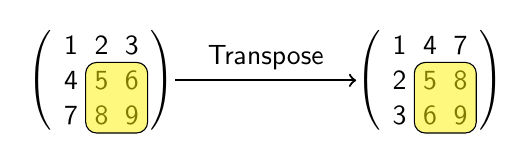
\begin{tikzpicture}
  \matrix[standard] (m)  {
       1 & 2 & 3 \\
       4 & 5 & 6 \\
       7 & 8 & 9 \\};
  \matrix[standard,right = 3cm of m] (n) {
       1 & 4 & 7 \\
       2 & 5 & 8 \\
       3 & 6 & 9 \\};
  \draw[->,shorten <=1em, shorten >=1em, thick]
    (m.east) to["Transpose"] (n);
\draw[submatrix] (m-2-2.north west) rectangle (m-3-3.south east);
\draw[submatrix] (n-2-2.north west) rectangle (n-3-3.south east);
\end{tikzpicture}
\end{document}
